\chapter{Analyse des Kontrollkanals}
\label{chap:4}
%
Ziel dieser Analyse ist es die benötigten Größen zur Bestimmung einer Normierungskonstante $\alpha$ für den Signalzerfall $\signal$ zu ermitteln. Diese ist in Gleichung~\eqref{eq:konst} definiert.
%
\begin{equation}
  \alpha=\frac{\mathcal{BR}(B^{+}\rightarrow\jpsi K^{+})\mathcal{BR}(\kontroll)}{N_{\kontroll}}\frac{(\epsilon_{\text{ges}})_{\kontroll}}{(\epsilon_{\text{ges}})_{\signal}}
  \label{eq:konst}
\end{equation}
%

Hierbei ist~$\mathcal{BR}(\kontroll)$ das bereits zu $\SI{5,986(33)}{\percent}$ \cite{pdg} vermessene Verzweigungsverhältnis für den Zerfall des $\jpsi$-Mesons in zwei Myonen. $\mathcal{BR}(B^{+}\rightarrow\jpsi K^{+})$ ist das zu $\SI{0.1027(31)}{\percent}$ \cite{pdg} bestimmte Verzweigungsverhältnis für den Zerfall eines $B$-Mesons in ein $\jpsi$- und ein $K$-Meson. $N_{\kontroll}$ beschreibt die in dieser Arbeit bestimmte Anzahl der gemessenen Signalereignisse für $B\rightarrow\jpsi(\rightarrow\mu\mu) K$.
$\epsilon_{\text{ges}}$ beschreibt die Gesamteffizienzen der Analyse des jeweiligen Kanals. Sie beinhalten die Detektion,
Rekonstruktion und Selektion der Ereignisse. Die Normierungskonstante ermöglicht es, systematische Fehler in der Bestimmung der
Signalkandidaten und Effizienzen des Signalzerfalls $\signal$ möglichst herauszukürzen und so ein deutlich exakteres Ergebnis
zu bestimmen. $\alpha$ kann dazu genutzt werden, zusammen mit der in \cite{ba-maik} ermittelten Anzahl erwarteter
Signalkandidaten eine Abschätzung für das Verzweigungsverhältnis des Zerfalls $\signal$ nach Gleichung~\eqref{eq:absch} zu ermitteln.
%
\begin{equation}
  \mathcal{BR}(\signal)<N_{\signal, \SI{95}{\percent}}\cdot\alpha\, .
  \label{eq:absch}
\end{equation}
%
Ideal wäre die Betrachtung eines Datensatzes für $\kontroll$. Hierzu existiert allerdings bisher keine Vorselektion für Daten des LHCb, da sich diese noch in Vorbereitung befindet. Daher wird ein Datensatz für den Zerfall $B^{+}\rightarrow\jpsi(\rightarrow\mu\mu) K^{+}$ verwendet.
Da die Selektion für die darin enthaltenen Ereignisse aufgrund der Abweichung vom Signalzerfall ebenfalls abweichend ist, müssen bestimmte Korrekturen der erwarteten Ereignisse durchgeführt werden. Diese werden in Abschnitt~\ref{sec:norm} diskutiert.
Um die benötigten Größen aus dieser Analyse zu bestimmen, wird eine schnittbasierte Selektion des Kontrollkanals
durchgeführt, um über die Ermittlung der rekonstruierten Signalereignisse und der dabei auftretenden Effizienzen
die Normierungskonstante bestimmen zu können.
%
%%%%%%%%%%%%%%%%%%%%%%%%%%%%%%%%%%%%%%%%%%%%%%%%%%%%%%%%%%%%%%%%%%%%%%%%%%%%%%%%%%%%%%%%%%%%%%%%%%%%%%%%%%%%%%%%%%
\section{Datensätze}
%%%%%%%%%%%%%%%%%%%%%%%%%%%%%%%%%%%%%%%%%%%%%%%%%%%%%%%%%%%%%%%%%%%%%%%%%%%%%%%%%%%%%%%%%%%%%%%%%%%%%%%%%%%%%%%%%%
%
Bei dem für die Analyse des Zerfalls $\kontroll$ verwendeten Datensatz handelt es sich um im Jahre 2012 am LHCb-Experiment bei einer Schwerpunkstenergie von $\sqrt{s}=\SI{8}{\tera\electronvolt}$ aufgenommene Daten, die einer integrierten Luminosität von $\SI{2}{\femto\barn^{-1}}$ entsprechen. Dazu ist eine dem Zerfall $B^{+}\rightarrow\jpsi(\rightarrow\!\mu\mu) K^{+}$ angepasste Selektion (Stripping \texttt{Bu2LLK\_mmLine}) verwendet worden, welche eine Effizienz von $\SI{8,744(6)}{\percent}$ aufweist. Die Selektionsvariablen und die zugehörigen Kriterien sind in Tabelle~\ref{tab:bstrip} aufgeführt.
%
\begin{table}[htb]
  \centering
  \caption{Auf den Datensatz angewendete Selektion.}
  \begin{tabular}{lc}
    \toprule
    Selektionsvariable                & Bedingung      \\
    \midrule
    $m_{B}$                           & $\in[\num{5129},\,\num{5429}]$ MeV/c²  \\
    $B^{+}:\chi_{\text{IP}}^2$        & $<\num{25}$  \\
    $B^{+}:\chi_{\text{VD,PV}}^2$     & $>\num{100}$  \\
    $B^{+}:\text{DIRA}$               & $>\num{0.9995}$  \\
    \bottomrule
  \end{tabular}
  \label{tab:bstrip}
\end{table}
%
Es wird also die rekonstruierte Masse des $B$-Mesons auf einen Bereich von $\pm\SI{150}{\mega\electronvolt}$ um die tatsächliche Masse von $\SI{5279.25(26)}{\mega\electronvolt}$ eingeschränkt. $\chi_{\text{IP}}^2$ ist dabei definiert als der Unterschied zwischen dem $\chi^2$ des Primärvertex' unter Berücksichtigung des beschriebenen Teilchens und jenem ohne Berücksichtigung desselben. Über $\chi_{\text{VD,PV}}^2$ wird die Flugdistanz des $B$-Mesons, die aufgrund seiner Lebensdauer entfernt vom Primärvertex liegt, nach unten beschränkt. Durch Wahl von Ereignissen mit $B^{+}:\text{DIRA}$ nahe $1$ werden solche selektiert, deren Winkel zwischen Impuls und rekonstruierter Spur des Teilchens möglichst gering und somit die Übereinstimmung möglichst groß ist.
Die verwendeten Daten enthalten dabei etwa 5959563 experimentell gemessene Daten, sowie etwa 2210052 in sogenannten Monte-Carlo-Simulationen generierte.\\

Monte-Carlo-Simulationen (MC) stellen eine bewährte Methode dar, um die Physik, die eine Theorie beschreibt und die experimentell gemessenen Daten vergleichbar zu machen. Um die Vorhersage für das Signal eines bestimmten Zerfalls in Form einer experimentellen Messung anzupassen, werden verschiedene Algorithmen zur Simulation der Kollisionen sowie deren Messung verwendet. Ziel ist es, die Kollision, anschließende Zerfälle sowie die Wechselwirkungen mit dem spezifischen Detektor möglichst exakt zu simulieren. So entsteht ein Signaldatensatz, welcher unter Anderem der Unterdrückung des experimentell gemessenen Untergrundes in Analysen, sowie der Suche nach neuer Physik dient. Bei dem hier verwendeten MC handelt es sich um die Simulation des Zerfalls $B^{+}\rightarrow\jpsi(\rightarrow\!\mu\mu) K^{+}$. Dabei werden die Proton-Proton-Kollisionen durch das Programm \texttt{PYTHIA 8.1} \cite{pythia} simuliert, welches über komplexe Modelle die entstehenden Teilchen generiert. Zerfallspunkte sowie die Produkte der bei diesen Kollisionen entstehenden $B$-Mesonen werden durch \texttt{EVTGEN} \cite{evtgen} simuliert. Die anschließende Wechselwirkug der Zerfallsprodukte mit dem Detektor konstruiert der Algorithmus \texttt{GEANT4}  \cite{geant4}, sodass die so entstandenen Datensätze durch dieselbe Hardware und Software (Trigger, Rekonstruktion etc.), wie die experimentell am LHCb Gemessenen laufen können. Die Umwandlung der berechneten Ereignisse in die dazu benötigten elektrischen Signale übernimmt die Software \texttt{BOOLE} \cite{boole}. Die Simulation geht dabei von einer Schwerpunktsenergie von $\sqrt{s}=\SI{8}{\tera\electronvolt}$ aus. Um die Simulation den Beschaffenheiten des Detektors anzupassen, ist der Winkelbereich der Zerfallsprodukte auf einen etwas größeren als den realen Akzeptanzbereich des Detektors beschränkt. Hierdurch werden Effekte am Rand des Detektors vernachlässigbar.
%%%%%%%%%%%%%%%%%%%%%%%%%%%%%%%%%%%%%%%%%%%%%%%%%%%%%%%%%%%%%%%%%%%%%%%%%%%%%%%%%%%%%%%%%%%%%%%
\section{Selektion des Kontrollkanals}
%%%%%%%%%%%%%%%%%%%%%%%%%%%%%%%%%%%%%%%%%%%%%%%%%%%%%%%%%%%%%%%%%%%%%%%%%%%%%%%%%%%%%%%%%%%%%%%
Die Datensätze für den zu untersuchenden Kontrollkanal $B^{+}\rightarrow\jpsi(\rightarrow\mu\mu) K^{+}$ werden zunächst schnittbasiert selektiert. Es erfolgt also eine Einschränkung auf den physikalisch für den gesuchten Zerfall relevanten Bereich. Dazu werden die in Tabelle~\ref{tab:strip} aufgeführten Bedingungen an die relevanten Ereignisse in dem Datensatz sowohl an die Daten, als auch an die Simulation gestellt. Diese Selektion orientiert sich dabei an der in der Studie zur Signaloptimierung \cite{ba-maik} angewendeten.

\begin{table}[htb]
  \centering
  \caption{Auf den Datensatz angewendete Selektion.}
  \begin{tabular}{lc}
    \toprule
    Selektionsvariable                & Bedingung      \\
    \midrule
    $m_{\mu\mu}$                      & $\in[\num{2946},\,\num{3176}]$ MeV/c²  \\
    $\mu^{-}:\chi_{\text{IP}}^2$      & $>\num{36}$  \\
    $\mu^{+}:\chi_{\text{IP}}^2$      & $>\num{36}$  \\
    $\mu^{-}:\text{GhostProb}$        & $<\num{0.3}$ \\
    $\mu^{+}:\text{GhostProb}$        & $<\num{0.3}$ \\
    $\jpsi:\text{BKGCAT}$(Nur MC)     & $==\num{0}$  \\
    $\jpsi:\text{DIRA}$               & $>\num{0}$  \\
    \bottomrule
  \end{tabular}
  \label{tab:strip}
\end{table}

Ziel dieser Selektion ist es, bei möglichst hoher Effizienz auf tatsächlich aus dem untersuchten Zerfall stammenden Ereignissen, möglichst viele Ereignisse aus sogenannten Untergrund-Zerfällen auszuschließen. Der bei allen Messungen unweigerlich in den Messungen dokumentierte Untergrund stellt eine Kombination verschiedener Teiluntergünde dar. Diese haben mitunter sehr unterschiedliche Ursachen. Der teilweise rekonstruierte Untergrund beispielsweise wird von Zerfällen induziert, die teilweise die selben Endprodukte wie der Signalzerfall erreichen, von denen allerdings nicht alle detektiert werden. Er überwiegt im unteren Massenfenster. Auch die Fehlerbehaftung der Messungen der einzelnen Detektorkomponenten erzeugt einen systematischen Untergrund, da die Messprozesse zwangsläufig statistischen Schwankungen unterliegen. Einen dritten Beitrag liefert der sogenannte kombinatorische Untergrund, der dadurch entsteht, dass beispielsweise zwei aus unabhängigen Zerfällen stammende Myonen, die zusammen zur Masse des $\jpsi$ kombiniert werden damit fälschlicherweise als Signal identifiziert werden.\\
Es wird zunächst ein Massenfenster von $m_{\mu\mu}=\SI{2946}{\mega\electronvolt}$ bis $m_{\mu\mu}=\SI{3176}{\mega\electronvolt}$ um die rekonstruierte Masse des $\jpsi$-Mesons von $\SI{3096.916(11)}{\mega\electronvolt}$ \cite{pdg} gelegt. Diese invariante Masse wird aus den Viererimpulsen der beiden Tochtermyonen berechnet, sodass durch das Fenster sichergestellt wird, dass diese auch aus einem $\jpsi$-Zerfall stammen. Die anderen Selektionsbedingungen sind aus einer rekursiven Optimierung des Signalzerfalls $\signal$ aus der parallel durchgeführten Studie \cite{ba-maik} übernommen, um eine optimale Vergleichbarkeit zu gewährleisten. Selbstverständlich sind sie für den Zerfall $\kontroll$ an die beiden Myonen angepasst.
Die Bedingungen $\mu^{\pm}:\chi_{\text{IP}}^2$ geben an, wie gut die rekonstruierten Myonen einem Primärvertex zugeordnet werden können. $\chi_{\text{IP}}^2$ ist dabei definiert als der Unterschied zwischen dem $\chi^2$ des Primärvertex' unter Berücksichtigung des beschriebenen
Teilchens und jenem ohne Berücksichtigung desselben \cite{chi2}. Die Variable $\mu^{\pm}:\text{GhostProb}$ gibt an, wie groß die Wahrscheinlichkeit
ist, dass die Identifikation eines Myons fälschlicherweise stattfand, sodass die Selektion diese Wahrscheinlichkeit auf maximal $\SI{30}{\percent}$
beschränkt. $\jpsi:\text{BKGCAT}$ legt fest, dass das in der Simulation rekonstruierte Ereignis auch als Signalereignis erzeugt wurde. Über die Variable $\jpsi:\text{DIRA}$ lässt sich die Übereinstimmung der Richtungen der aus den Vertices rekonstruierten Spuren sowie den Impulsen derselben Teilchen prüfen. Da es sich um den $cosinus$ des Winkels zwischen diesen Richtungen handelt, sollte diese Variable möglichst nahe bei $1$ liegen. Nach Anwenden der so gewählten Selektion auf die Simulation bleiben 1814293 Ereignisse. Die Effizienz dieser Selektion folgt daher nach Gleichung~\eqref{eq:eff_strip1}. Die Fehlerangaben entsprechen dabei den Binomial-Fehlern.
%
\begin{equation}
  \epsilon_\text{Selektion}=\frac{N_\text{MC-events after selection}}{N_\text{MC-events after strip}}=\SI{82.09(3)}{\percent} \, .%\frac{1814293}{2210052}
  \label{eq:eff_strip1}
\end{equation}
%
Des Weiteren werden sogenannte Triggerstufen als Bedingung für die Selektion der relevanten Ereignisse herangezogen. Die Trigger fungieren als Entscheidungskriterien dafür, ob ein Ereignis potentiell interessante Physik bereithält und somit vom Detektor aufgenommen und gespeichert werden soll, oder nicht. Die \texttt{TOS}-Trigger (\textit{triggered on signal}) lösen dabei aus, wenn Teilchen aus Signalzerfällen detektiert werden. Die hier, sowie in der Signalanalyse \cite{ba-maik} verwendeten Trigger gliedern sich in die in Tabelle~\ref{tab:trigger} aufgeführten drei Stufen \texttt{L0}, \texttt{HLT1} und \texttt{HLT2}. Diese sortieren nacheinander Ereignisse heraus, die nicht mindestens eine der aufgeführten Bedingungen innerhalb einer Stufe erfüllen. Daher selektiert jede Stufe feiner als die Vorherige.
%
\begin{table}[htb]
  \centering
  \caption{Auflistung der auf das $\jpsi$-Meson angewandten Trigger.
  Ereignisse, die nicht innerhalb jeder einzelnen Triggerstufe mindestens eine Triggerbedingung erfüllen, werden aussortiert.}
  \begin{tabular}{l}
    \toprule
    \textbf{L0-Trigger}                                 \\
    \quad\texttt{L0MuonDecision\_TOS}              \\
    \quad\texttt{L0HadronDecision\_TOS}            \\
    \midrule
    \textbf{HLT1-Trigger}                               \\
    \quad\texttt{Hlt1TrackAllL0Decision\_TOS}      \\
    \quad\texttt{Hlt1TrackMuonDecision\_TOS}       \\
    \midrule
    \textbf{HLT2-Trigger}                               \\
    \quad\texttt{Hlt2Topo2BodyBBDTDecision\_TOS}   \\
    \quad\texttt{Hlt2Topo3BodyBBDTDecision\_TOS}   \\
    \quad\texttt{Hlt2Topo4BodyBBDTDecision\_TOS}   \\
    \quad\texttt{Hlt2TopoMu2BodyBBDTDecision\_TOS} \\
    \quad\texttt{Hlt2TopoMu3BodyBBDTDecision\_TOS} \\
    \quad\texttt{Hlt2TopoMu4BodyBBDTDecision\_TOS} \\
    \bottomrule
  \end{tabular}
  \label{tab:trigger}
\end{table}
%
Die Effizienz $\epsilon$ dieser drei Triggerstufen, sowie der Selektion bezogen auf die Zahl der Ereignisse im Datensatz beträgt für die Simulation den in Gleichung~\eqref{eq:eff_ges1} aufgeführten Wert.
%
\begin{equation}
  \epsilon_\text{Trigger}=\frac{N_\text{MC-events after trigger}}{N_\text{MC-events after selection}}=\SI{74.15(4)}{\percent} \, .% \frac{1345240}{1814293}
  \label{eq:eff_ges1}
\end{equation}
%
Zusammen mit der Generatoreffizienz
%
\begin{equation}
  \epsilon_\text{gen}=\frac{N_\text{Akzeptanz}}{N_\text{wahr}}=\SI{16.099(21)}{\percent}
\end{equation}
%
und der Strippingeffizienz $\epsilon_\text{strip}=\SI{8.744(6)}{\percent}$ kann so die Gesamteffizienz wie in Gleichung~\eqref{eq:eff_ges} berechnet werden.
%
\begin{equation}
  \epsilon_{\kontroll, \text{ges}}
  =\epsilon_\text{gen}\cdot\epsilon_\text{strip}\cdot\epsilon_\text{Selektion}\cdot\epsilon_\text{Trigger}=\SI{0.857(1)}{\percent}
  \label{eq:eff_ges}
\end{equation}
%%%%%%%%%%%%%%%%%%%%%%%%%%%%%%%%%%%%%%%%%%%%%%%%%%%%%%%%%%%%%%%%%%%%%%%%%%%%%%%%%%%%%%%%%%%%%%%
\section{Massenfit}
\label{sec:massenfit}
%%%%%%%%%%%%%%%%%%%%%%%%%%%%%%%%%%%%%%%%%%%%%%%%%%%%%%%%%%%%%%%%%%%%%%%%%%%%%%%%%%%%%%%%%%%%%%%
Um aus dem so eingeschränkten und selektierten MC-Datensatz die Anzahl der Signalkandidaten $N_{\kontroll}$ zu bestimmen, wird ein sogennanter \textit{extended maximum-likelihood-fit} \cite{extended} der rekonstruierten $\jpsi$-Masse durchgeführt. Die oben
beschriebene Selektion beschränkt den Massenbereich des rekonstruierten $\jpsi$-Mesons auf einen Bereich von etwa
$[m_{\mu\mu}-\SI{150}{\mega\electronvolt}, m_{\mu\mu}+\SI{80}{\mega\electronvolt}]$. Die Masse des $\jpsi$-Mesons beträgt $\SI{3096.916(11)}{\mega\electronvolt}$ \cite{pdg}. Diese Einschränkung konzentriert den Fit auf die $\SI{60.87}{\percent}$ der gesamten Ereignisse, welche in diesem Bereich liegen, da so das gesamte Signal, aber möglichst wenig Untergrund vorliegen. Gleichzeitig ist das Intervall weit genug gewählt, um auch den eingangs dieses Kapitels beschriebenen Untergrund modellieren zu können. Da das hier verwendete Modelle numerisch sehr stark von der Wahl der Startwerte und der Iterationsintervalle abhängt, wird die Ausgleichsrechnung auf einem auf zufällig ausgewählte $100\,000$ Ereignisse beschränkten Teil des Gesamtdatensatzes durchgeführt. Hieraus folgt demnach ein Skalierungsfaktor von $13,4524$ für die bestimmten Signalereignisse. \\
%
Mit Hilfe des frameworks \texttt{RooFit} \cite{roofit} wird die Verteilung der rekonstruierten $\jpsi$-Masse an ein Gesamtmodell angepasst. Dazu wird für ein aus Signalfunktion und Untergrundfunktion zusammengesetztes Modell der in Gleichung~\ref{eq:massenfit} dargestellten Form eine Ausgleichrechnung durchgeführt.
%
\begin{equation}
  \symup{G}(m_{\mu\mu})= \symup{S}(m_{\mu\mu}) + \symup{B}(m_{\mu\mu})
  \label{eq:massenfit}
\end{equation}
%
$\symup{S}(m_{\mu\mu})$ beschreibt hierbei das verwendete Signalmodell, während $\symup{B}(m_{\mu\mu})$ den Untergrund modelliert. Die Verteilung der Massen entspricht in etwa einer Gaußverteilung, zeigt aber an den Rändern sogenannte \textit{Ausläufer}: nicht der Normalverteilung entsprechende, beispielsweise durch Polynome beschriebende Verteilungen. Diese werden unter Anderem durch die Abstrahlung von niederenergetischen Photonen in Form von \textit{final state radiation} erzeugt \cite{cb}. Um diese Eigenschaft der Verteilung hinreichend zu modellieren, werden sogenannte \textit{Crystal Ball}-Funktionen (CB) verwendet. Diese zur Modellation asymmetrischer Wahrscheinlichkeitsverteilungen verwendeten Funktionen stellen eine Gaußfunktion dar, welche an einer Seite in eine Potenzfunktion übergeht. Die Darstellung ist in Gleichung~\ref{eq:cb} \cite{cb} angegeben, wobei die Parameter $A$ und $B$ stets so bestimmt werden, dass die Funktion analytisch ist.
%
\begin{equation}
  {\displaystyle CB(x;\alpha ,n,{\mu},\sigma,N)=N\cdot {\begin{cases}\exp \left(-{\frac {(x-{\mu})^{2}}{2\sigma ^{2}}}\right),&{\mbox{falls }}{\frac {x-{\mu}}{\sigma }}>-\alpha \\A\cdot \left(B-{\frac {x-{\mu}}{\sigma }}\right)^{-n},&{\mbox{falls }}{\frac {x-{\mu}}{\sigma }}\leqslant -\alpha \end{cases}}}
  \label{eq:cb}
\end{equation}
%
Als Modell für den Untergrund in dieser Messung wird ein exponentieller Zusammenhang der in Gleichung~\ref{eq:exp} dargestellten Form verwendet.
%
\begin{equation}
  B(x; c)= \symup{e}^{c\cdot x} \, .
  \label{eq:exp}
\end{equation}
%
Da durch nicht gaußverteilte Detektoreffekte \textit{Ausläufer} auch bei höheren Energien entstehen, kann es sinnvoll sein, durch die Kombination von zwei CB-Funktionen, also einem \textit{Double-Crystal-Ball} (DCB) die Modellation dieser zu ermöglichen \cite{ipatia}.
Im Folgenden wird der Signalteil der Verteilung der rekonstruierten Masse also als DCB-Funktion modelliert. Dies entspricht einem Gesamtmodell der in Gleichung~\ref{eq:dcb} dargestellten Form.
%
\begin{equation}
  \begin{split}
  \symup{G}(m_{\mu\mu}; f)={}&\symup{CB}_1(m_{\mu\mu};\alpha_1,\mu,\sigma_1,n_1) + f\symup{CB}_2(m_{\mu\mu};\alpha_2,\mu,\sigma_2,n_2)\\ &+ \symup{B}(m_{\mu\mu};c)
  \end{split}
  \label{eq:dcb}
\end{equation}
%
Der Faktor $f$ beschreibt dabei das Verhältnis der beiden CB-Funktionen und liegt zwischen 0 und 1. Zu dieser Funktion wird der oben beschriebene exponentielle Untergrund ($\symup{B}(m_{\mu\mu})$) hinzugefügt und das so entstehende Gesamtmodell an die Daten angepasst. Dazu werden die in Gleichung~\eqref{eq:dcb} aufgeführten Parameter mit Hilfe von \texttt{RooFit} der Verteilung angepasst.
%
%
%\begin{table}[H]
%  \centering
%  \caption{Auflistung der für den Fit des Signalmodells verwendeten Parameter.}
%  \begin{tabular}{ccc}
%    \toprule
%    \textbf{Crystall Ball 1}    & \textbf{Crystall Ball 2} & Intervall für den Fit \\
%    \midrule
%    $\alpha_1$                  & $\alpha_2$               & [-4, 0], [0, 4] \\
%    $\mu$                       & $\mu$                    & [2946, 3176] \\
%    $\sigma_1$                  & $\sigma_2$               & [1, 20], [1, 20] \\
%    $n_1$                       & $n_2$                    & [0, 20], [0, 20] \\
%    \bottomrule
%  \end{tabular}
%  \label{tab:params}
%\end{table}
%
$\alpha$ gibt dabei an, ab wann die Gaußverteilung durch den Potenzzusammenhang ersetzt wird. Dies beeinflusst also, wann die Modellation der \textit{Ausläufer}
einsetzt. Ein positives $\alpha$ bedeutet dabei, dass der \textit{Ausläufer} zu kleineren Werten einsetzt, während ein $\alpha<0$
diesen zu größeren Werten modelliert. $\mu$ beschreibt den Wert für das Maximum der Gaußfunktion. Anschaulich beschreibt dies die aus
den Daten rekonstruierte Masse des $\jpsi$-Mesons. Da beide \textit{Crystal Ball}-Funktionen an den gleichen gaußschen Teil der Verteilung angepasst werden,
wird über diesen Parameter für beide Funktionen gemeinsam iteriert. Das $\sigma$ gibt wie bei gaußschen Verteilungen üblich die Breite der Verteilung an. Über den Parameter $n$ kann das Modell für den \textit{Ausläufer} angepasst werden. Der Wert für $n$ gibt den Grad der Potenz an.
Die Ausgleichsrechnung ergibt die in Tabelle~\ref{tab:fit1} dargestellten Werte für die Parameter. Die Ausgleichsrechnung ist so durchgeführt, dass alle Parameter bis auf $n_2$ frei sind. Diese Einschränkung ist notwendig, damit die Ausgleichsrechnung auf dem hier vorliegenden Datensatz konvergiert und die Ergebnisse sowie die Fehler stabile Werte annehmen. Der Wert wurde durch schrittweise Annäherung in eigenen Studien bestimmt. Eine Anpassung der Startwerte und Iterationsintervalle böte an diesem Punkt Potential für eine exaktere Untersuchung. Die so definierte Gesamtfunktion, sowie die einzelnen Komponenten sind in Abbildung~\ref{fig:fit1} dargestellt. Die Wahl mehrerer CB-Funktionen ermöglicht es unter anderem, die Gaußverteilung, also den Kern des Fits zu verzerren. Auf diese Weise, ist das Gesamtmodell in der Lage auch nicht gaußverteilte Verteilungen in diesem Bereich zu modellieren. Allerdings ist die Ausgleichsrechnung mit \texttt{RooFit} für Modelle dieser Art numerisch sehr instabil, sodass die Wahl der Intervalle und Startwerte für die freien Parameter großen Einfluss auf das Ergebnis hat. Daher ist eine systematische und zuvor genau zu untersuchende Bestimmung dieser von Nöten, welche über den in dieser Arbeit gesteckten Rahmen hinaus ginge.
%
\begin{table}[H]
  \centering
  \caption{Auflistung der Fit-Ergebnisse des Signalmodells (DCB), sowie des exponentiellen Hintergrunds. Der Parameter $n_2$ ist hier auf einen Wert von 40 festgesetzt.}
  \begin{tabular}{lr@{$\,\pm\,$}l}
    \toprule
    \textbf{Signalmodell}         &  \multicolumn{2}{c}{Fit-Ergebnis} \\
    \midrule
    \quad$\alpha_1$               & 1,78    & 0,05 \\
    \quad$\mu$                    & 3097,71 & 0,05 \\
    \quad$\sigma_1$               & 10,0    & 0,2 \\
    \quad$n_1$                    & 1,10    & 0,05 \\
    \quad$\alpha_2$               & -1,87   & 0,08 \\
    \quad$\sigma_2$               & 15,6    & 0,4 \\
    \quad$f$                      & 0,39    & 0,03 \\
    \quad$n_\text{BKG}$           & 303     & 135 \\
    \quad$n_\text{Sig}$           & 99700   & 334 \\
    \midrule
    \textbf{Untergrundmodell}     &  \multicolumn{2}{c}{Fit-Ergebnis} \\
    \midrule
    \quad$c$                      & $-1,1\cdot10^{-6}$   & $4,5\cdot10^{-3}$ \\
    \bottomrule
  \end{tabular}
  \label{tab:fit1}
\end{table}
%
\begin{figure}[H]
  \centering
      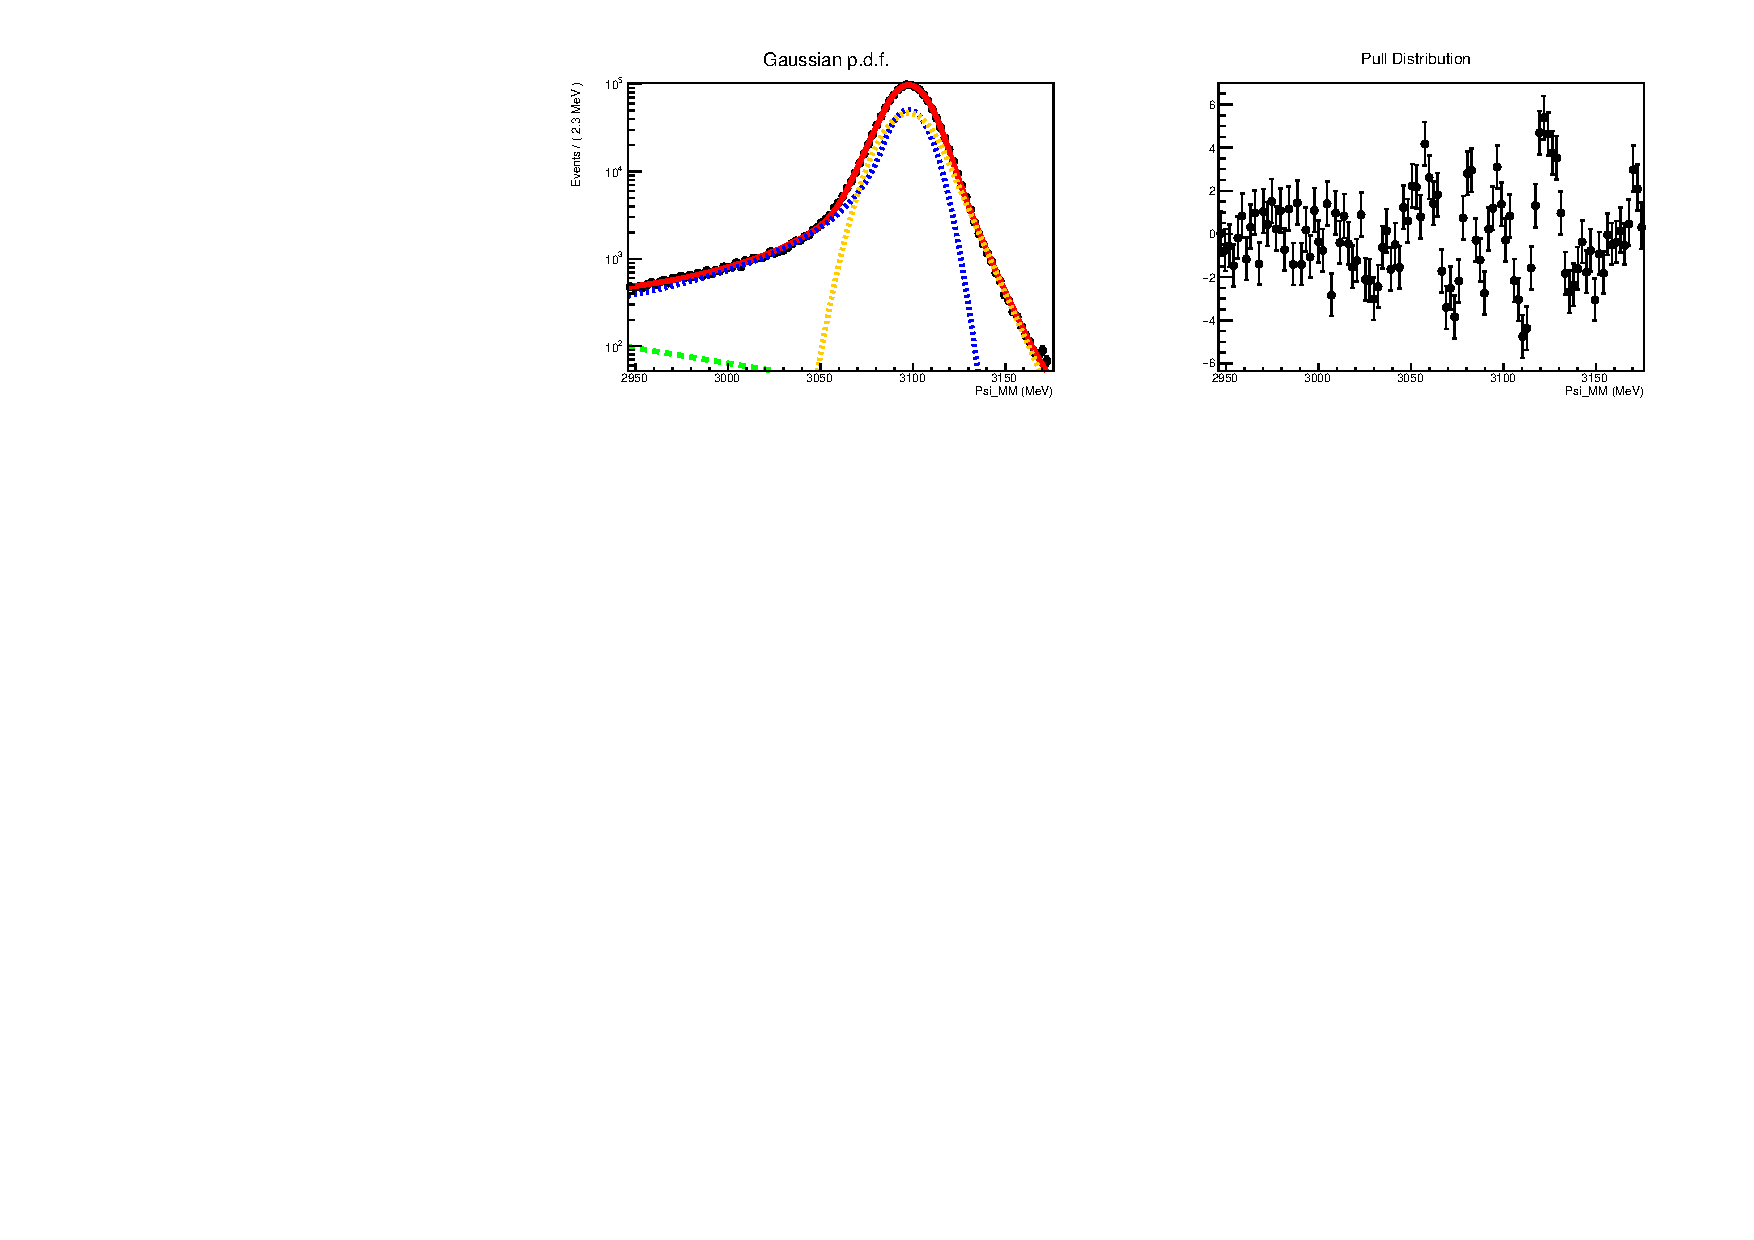
\includegraphics[width=0.8\textwidth]{Plots/DCBexp.pdf}
  \caption{Verteilung der $\jpsi$-Masse sowie das Ergebnis des DCB-Fits. (schwarz: Daten, grün: Untergrund, rot: Gesamtmodell, blau: CB1, orange: CB2).}
  \label{fig:fit1}
\end{figure}
%
Über die Skalierung mit dem Faktor $13,4524$ folgen für die Anzahl der Signal- sowie der Untergrundereignisse $n_\text{Sig, skaliert}=1341204\,\pm\,4493$ und $n_\text{BKG, skaliert}=4076\,\pm\,1816$. Diese sind als Parameter für die Kombination aus Untergrund- und Signalmodell über die Ausgleichsrechnung bestimmt worden und entsprechen der durch dieses Modell dargestellten Verteilung der Signalereignisse bzw. der Untergrundereignisse.\\
%%%%%%%%%%%%%%%%%%%%%%%%%%%%%%%%%%%%%%%%%%%%%%%%%%  IPATIA  %%%%%%%%%%%%%%%%%%%%%%%%%%%%%%%%%%%%%%%%%%%%%%%%%%%%%%%%%%%%%%
Um der oben beschriebenen numerischen Instabilität vorzubeugen, kann beispielsweise die sogenannte IPATIA-Funktion als Signalmodell verwendet werden. Diese ist in Referenz~\cite{ipatia} genau beschrieben. Das ihr zugrunde liegende Modell berücksichtigt die oben erwähnten \textit{Ausläufer} und ermöglicht die Verzerrung der gaußschen 'Kernverteilung'. Die Funktionsvorschrift hat die in Gleichung~\ref{eq:ipatia} dargestellte Form.
%
\begin{equation}
  \begin{split}
  &\symup{I}(m,\mu,\sigma,\lambda,\zeta,\beta,a,n)\propto\\
    &\begin{cases}
      \begin{split}
      ((m-\mu)^2&+A_\lambda²(\zeta)\sigma²)^{\frac{1}{2}\lambda-\frac{1}{4}}\symup{e}^{\beta(m-\mu)}\\
      &\cdot K_{\lambda-\frac{1}{2}}\left(\zeta\sqrt{1+(\frac{m-\ mu}{A_\lambda(\zeta)\sigma})^2}\right),
      \end{split} & \text{wenn} \frac{m-\mu}{\sigma}>-a \\
      \frac{G(\mu-a\sigma,\mu,\sigma,\lambda,\zeta,\beta)}{\left(1-m\/(n\frac{G(\mu-a\sigma,\mu,\sigma,\lambda,\zeta,\beta)}{G'(\mu-a\sigma,\mu,\sigma,\lambda,\zeta,\beta)}-a\sigma)\right)^n} ,& \text{sonst}
    \end{cases}
  \end{split}
  \label{eq:ipatia}
\end{equation}
%
Die Funktion $G(\mu-a\sigma,\mu,\sigma,\lambda,\zeta,\beta)$ ist dabei der für $\frac{m-\mu}{\sigma}>-a$ definierte Zusammenhang. Bei $K$
handelt es sich um Bessel-Funktionen dritter Gattung. $A_\lambda$ steht der Übersichtlichkeit halber als Abkürzung für
%
\begin{align*}
  A_\lambda^2=\frac{\zeta K_\lambda(\zeta)}{K_{\lambda+1}(\zeta)}\; .
\end{align*}
%
Die Ipatia-Funktion modelliert die Verteilung der rekonstruierten Masse sowohl im Bereich der $\jpsi$-Masse, als auch im Bereich der \textit{Ausläufer} äußerst exakt. Allerdings ist auch hier die Wahl der Startwerte für die Iterationen entscheidend für die Konvergenz der Ausgleichsrechnung. Eine systematische Bestimmung solcher Startwerte ginge über den Rahmen dieser Bachelorarbeit hinaus; prinzipiell stellt die Durchführung einer solchen Ausgleichsrechnung allerdings eine Möglichkeit der Weiterführung dieser Analyse dar. Eine grobe Ausgleichrechnung ist in Abbildung~\ref{fig:fit2} dargestellt. Es zeigt sich, dass der Fit schon in diesem frühen Stadium der Massenverteilung sehr gut entspricht.
%
\begin{figure}[H]
  \centering
      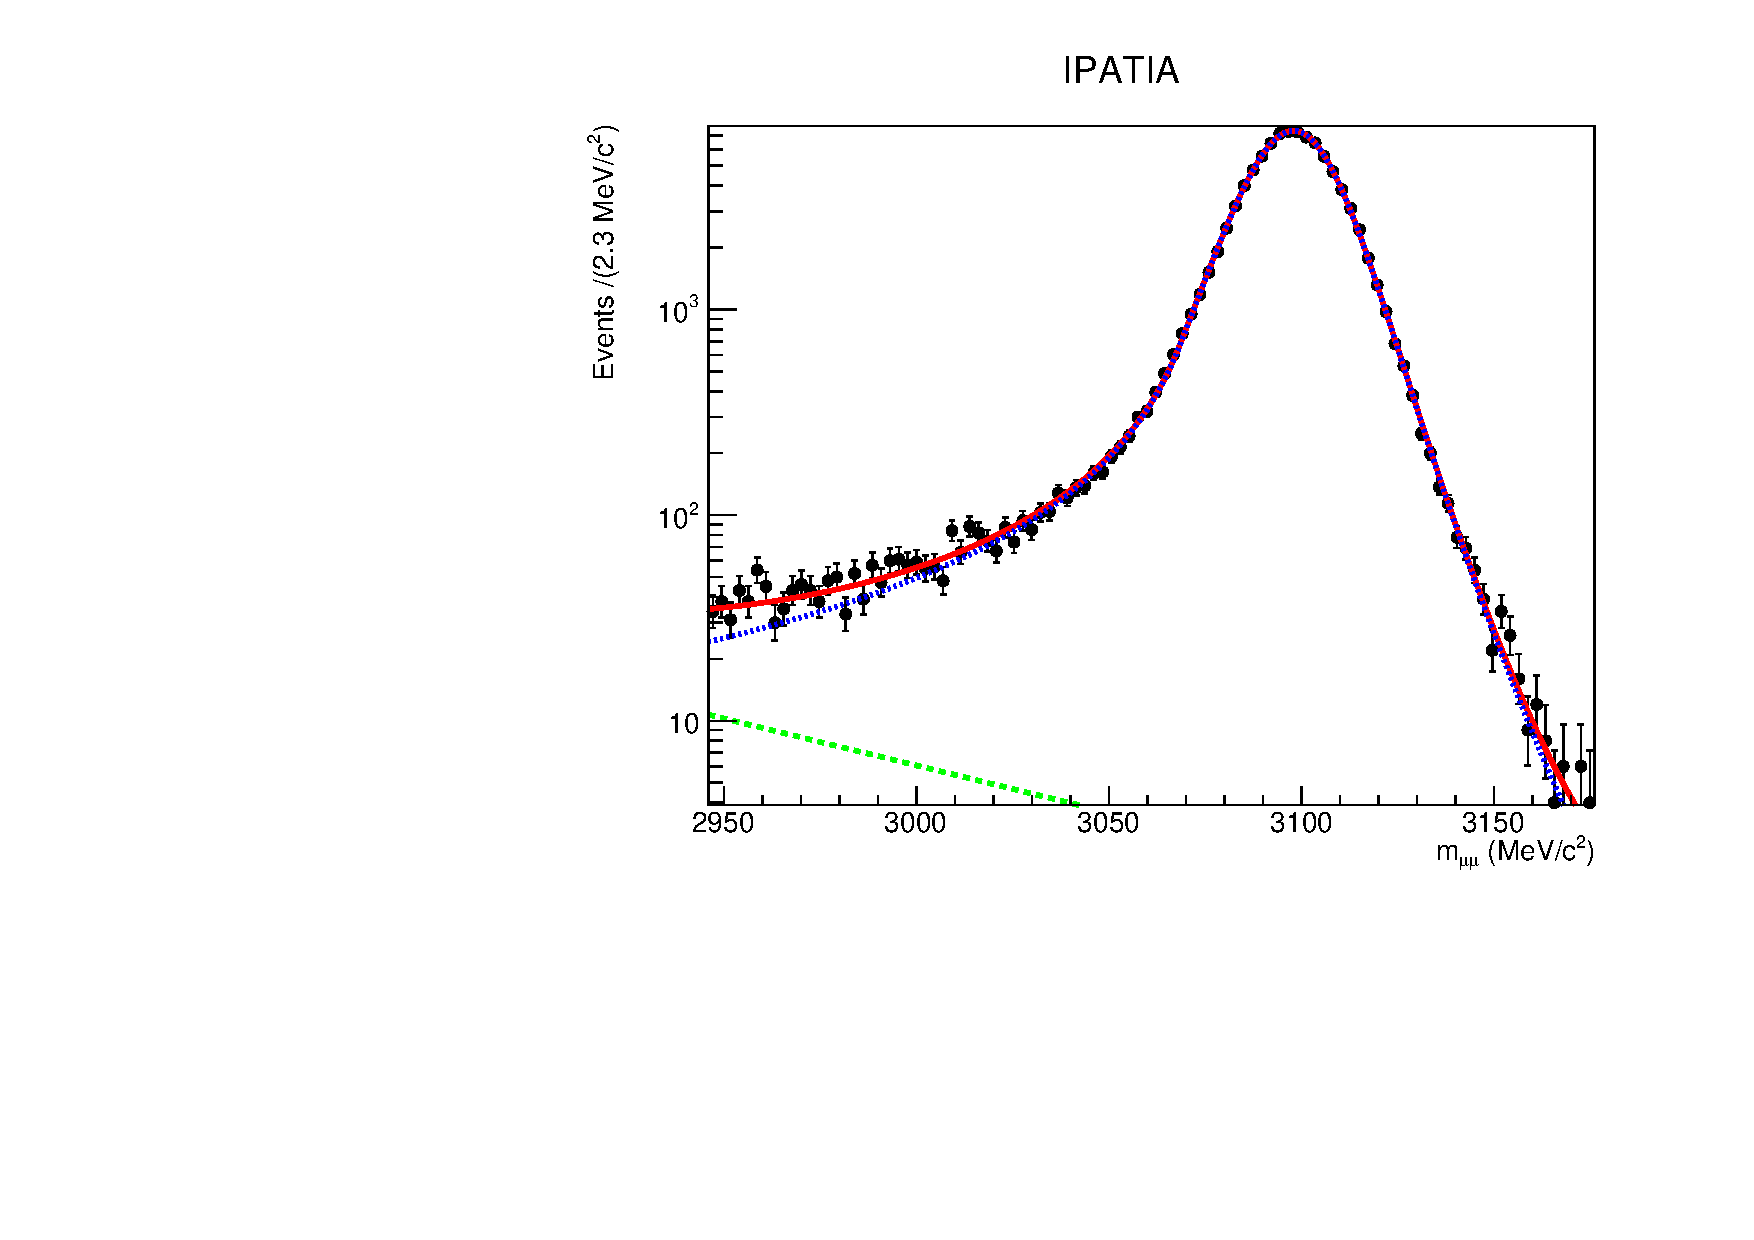
\includegraphics[width=0.8\textwidth]{Plots/IPATIAexp.pdf}
  \caption{Verteilung der $\jpsi$-Masse sowie eine grobes Fit-Ergebnis für die IPATIA-Funktion. (grün: Untergrund, rot: Gesamtmodell, blau: IPATIA).}
  \label{fig:fit2}
\end{figure}
%%%%%%%%%%%%%%%%%%%%%%%%%%%%%%%%%%%%%%%%%%%%%%%%%%%%%%%%%%%%%%%%%%%%%%%%%%%%%%%%%%%%%%%%%%%%%%%
\section{Bestimmung der Signalkandidaten}
%%%%%%%%%%%%%%%%%%%%%%%%%%%%%%%%%%%%%%%%%%%%%%%%%%%%%%%%%%%%%%%%%%%%%%%%%%%%%%%%%%%%%%%%%%%%%%%
Die in Abschnitt~\ref{sec:massenfit} durchgeführte Ausgleichsrechnung ermöglicht die Abschätzung der Anzahl der Signalkandidaten für $\kontroll$. Diese folgt aus dem Ergebnis für die Ausgleichsrechnung des \textit{Double Crystal Ball}-Modells. Es ergibt sich der in Gleichung~\eqref{eq:nkontroll} beschriebene Wert.
%
\begin{equation}
  N_{\kontroll}=1\,341\,204\,\pm\,4493
  \label{eq:nkontroll}
\end{equation}
%
Die Zahl der Signalkandidaten beträgt damit $\SI{99,7(3)}{\percent}$ der in dem Datensatz nach der Selektion noch enthaltenen Ereignisse.
%%%%%%%%%%%%%%%%%%%%%%%%%%%%%%%%%%%%%%%%%%%%%%%%%%%%%%%%%%%%%%%%%%%%%%%%%%%%%%%%%%%%%%%%%%%%%%%
\section{Bestimmung der Normierungskonstante}
\label{sec:norm}
%%%%%%%%%%%%%%%%%%%%%%%%%%%%%%%%%%%%%%%%%%%%%%%%%%%%%%%%%%%%%%%%%%%%%%%%%%%%%%%%%%%%%%%%%%%%%%%
Aus der parallel durchgeführten Analyse \cite{ba-maik} wird die Gesamteffizienz für die Bestimmung der Signalkandidaten zu
%
\begin{equation}
  \epsilon_{\signal, \text{tot}}=(1,2\,\pm\,0,4)\cdot 10^{-6}
\end{equation}
%
referenziert. Das Verzweigungsverhältnis für den Zerfall $\kontroll$ ist zu \\$\SI{5,961(33)}{\percent}$ und das für den Zerfall $B\rightarrow\jpsi X$ zu $\SI{1,094(32)}{\percent}$ bestimmt \cite{pdg}. Der in
dieser Analyse verwendete Datensatz unterscheidet sich von dem in der Analyse \cite{ba-maik} verwendeten in der Vorselektion. Die
Kandidaten für den Zerfall $\kontroll$ werden so selektiert, dass die Impulse der beiden Myonen die Masse des $\jpsi$-Mesons
rekonstruieren und dass das $\jpsi$-Meson zusammen mit dem $K^+$ aus dem Zerfall eines $B$-Mesons stammt. Für die Selektion der Kandidaten für $\signal$ werden zwar auch Elektron-Myon-Paare gesucht, deren Impulse die Masse des $\jpsi$-Mesons rekonstruieren, allerdings wird
hier nicht die Rekonstruktion zu einem $B$-Meson vorgenommen. Sie wird dadurch ersetzt, dass der Zerfallsvertex der Myonen nicht direkt
am Kollisionspunkt liegen darf. Da dieser Unterschied Einfluss auf die Zahl der Signalkandidaten hat, bedarf es einer Korrektur.
%Eine Korrektur der Anzahl der ermittelten Signalkandidaten kann über den in Gleichung~\eqref{eq:korrektur} definierten Zusammenhang mit Hilfe des Faktors $R$ erfolgen.
%
%\begin{equation}
%  N_\text{korr}=N_{\kontroll}\cdot\underbrace{\frac{\sigma(pp\rightarrow\jpsi)}{\sigma(pp\rightarrow B^+)}}_{R_1}
%  \label{eq:korrektur}
%\end{equation}
%%
%Das Verhältnis aus $\sigma(pp\rightarrow\jpsi)$ und $\sigma(pp\rightarrow B^+)$ spiegelt hierbei ein Maß für die
%Produktionswahrscheinlichkeit der beiden Mesonen wider. Dadurch wird die zusätzliche Beschränkung der $\kontroll$-Kandidaten auf die Herkunft aus einem B-Zerfall ausgeglichen. Der Wirkungsquerschnitt $\sigma(pp\rightarrow\jpsi)$ ist dabei Messungen der LHCb Kollaboration entnommen \cite{sigmajpsi} und beträgt $\SI{1.14(16)}{\micro\barn}$; der Wirkungsquerschnitt $\sigma(pp\rightarrow B^+)$ entspricht dem in \cite{sigmaB} gemessenen und ist zusätzlich über einen Faktor von $\sfrac{8}{7}$ auf die Schwerpunktsenergie von $\SI{8}{\tera\electronvolt}$ skaliert. Er beträgt $\SI{44.46(324)}{\micro\barn}$. Der Korrekturfaktor berechnet sich gemäß Gleichung~\eqref{eq:korrfaktor}.
%%
%\begin{equation}
%  R_1=\frac{\sigma(pp\rightarrow\jpsi)}{\sigma(pp\rightarrow B^+)}=0,026\,\pm\,0,004
%  \label{eq:korrfaktor}
%\end{equation}
%%
%Die so korrigierte Zahl an Signalereignissen entspricht
%%
%\begin{equation}
%  N_\text{korr}=(34000\,\pm\,5000)\; .
%\end{equation}
%%
%Da die bei dieser Korrektur verwendeten Wirkungsquerschnitte mit nicht zu vernachlässigenden Fehlern behaftet sind, kann
%zum Vergleich des Ergebnisses der Korrekturfaktor über eine weitere Methode bestimmt werden.
%

Dazu wird zunächst über die in dieser Arbeit bestimmte Anzahl an $\kontroll$ Zerfällen auf die Zahl der insgesamt erzeugten $B^{+}$-Mesonen zurückgerechnet. Diese Zahl folgt über den in Gleichung~\eqref{eq:nb+} definierten Zusammenhang.
%
\begin{equation}
  \begin{split}
  N_{B^{+}}=&\frac{N_{\kontroll}}{\mathcal{BR}(B^{+}\rightarrow\jpsi K^{+})\mathcal{BR}(\kontroll)}\cdot\frac{1}{(\epsilon_\text{ges})_{\kontroll}}\\
  =&(2,56\,\pm\,0,08)\cdot10^{12}
  \end{split}
  \label{eq:nb+}
\end{equation}
%
Die Zahl der $B^{-}$-Mesonen entspricht der der $B^{+}$-Mesonen. Unter der Annahme, dass die Zahl der $B^0$ in etwa der der $B^{+}$ entspricht (also $f_u\approx f_d$), folgt die Zahl beider $B$-Mesonen als das Doppelte, der in Gleichung~\eqref{eq:nb+} bestimmten Zahl. Schließlich muss die bestimmte Zahl noch um die in Gleichung~\eqref{eq:bs} definierte Zahl der $B_s$-Mesonen erweitert werden; wieder unter der Annahme, dass
$f_u\approx f_d$. Auch hier berücksichtigt ein Faktor $2$ das ladungskonjugierte Teilchen. Das Verhältnis, in welchem diese im Vergleich zu $B_0$-Mesonen produziert werden entspricht in etwa dem in dieser Gleichung angegebenen Faktor $\sfrac{f_s}{f_d}=0,267\,\pm\,0,020$ \cite{fs}.
%
\begin{equation}
  N_{B_s}\approx N_{B^+}\cdot\frac{f_s}{f_u} = N_{B^0}\cdot\frac{f_s}{f_d}=(6.8\,\pm\,0.6)\cdot10^{11}
  \label{eq:bs}
\end{equation}
%
Aus diesem Wert lässt sich dann über das Verzweigungsverhältnis für den Zerfall in $\jpsi$-Mesonen die korrigierte Zahl der Signalkandidaten bestimmen. Die so bestimmte, korrigierte Zahl der $\jpsi$-Mesonen folgt damit nach Gleichung~\eqref{eq:jpsi}.
%
\begin{equation}
  N_\text{korr}=(2N_{B^{+}}+2N_{B_s}+N_{B^{0}})\cdot\mathcal{BR}(B\rightarrow\jpsi X)=(9,9\,\pm\,0,4)\cdot10^{10}
  \label{eq:jpsi}
\end{equation}
%
Über den eingangs beschriebenen Zusammenhang~\eqref{eq:konst} für die Normierungskonstante und $\mathcal{BR}(B^{+}\rightarrow\jpsi K^{+}) = \SI{0.1027(31)}{\percent}$ \cite{pdg} kann diese nun mit Hilfe der bestimmten Werte berechnet werden:
%
\begin{align*}
  \alpha=&\frac{1}{N_\text{korr}\cdot(\epsilon_{\text{ges}})_{\signal}} \\
  =&\,(1,3\,\pm\,0,4)\cdot10^{-5}\\
\end{align*}
%%%%%%%%%%%%%%%%%%%%%%%%%%%%%%%%%%%%%%%%%%%%%%%%%%%%%%%%%%%%%%%%%%%%%%%%%%%%%%%%%%%%%%%%%%%%%%%
\section{Obere Abschätzung für das Verzweigungsverhältnis}
%%%%%%%%%%%%%%%%%%%%%%%%%%%%%%%%%%%%%%%%%%%%%%%%%%%%%%%%%%%%%%%%%%%%%%%%%%%%%%%%%%%%%%%%%%%%%%%
Die Normierungskonstante $\alpha$ ermöglicht nun zusammen mit der in der Analyse des Zerfalls $\signal$ bestimmten Anzahl an Signalkandidaten das Bestimmen einer oberen Abschätzung für das Verzweigungsverhältnis $\mathcal{BR}(\signal)$. Dieses berechnet sich gemäß des in Gleichung~\eqref{eq:absch} angegebenen Zusammenhanges zu:
%
\begin{equation}
  \begin{split}
    \mathcal{BR}(\signal)<N_{\signal, \SI{95}{\percent}}\cdot\alpha=& (7\,\pm\,1)\cdot((1,3\,\pm\,0,4)\cdot10^{-5})\\=& (9,2\,\pm\,3,4)\cdot10^{-5} \, .
  \end{split}
\end{equation}
%

\nocite{biblatex, make, toolbox, gitbash, siunitx}
